\documentclass[preprint,numbers,10pt]{sigplanconf}

\usepackage[hidelinks]{hyperref}
\usepackage{graphicx}
\usepackage{xcolor}
\usepackage{float}
\newcommand\comment[1]{\textcolor{blue}{#1}}

\newcommand\markus[1]{\textcolor{red}{MARKUS: {#1}}}
\newcommand\federico[1]{\textcolor{red}{FEDERICO: {#1}}}
\newcommand\ana[1]{\textcolor{red}{ANA: {#1}}}

\begin{document}

\title{Language Workbench Challenge 2016: the JetBrains MetaProgramming System}

\authorinfo{Eugen Schindler}{Canon/Oc\'e Technologies}{eugenschindler@gmail.com}
\authorinfo{Klemens Schindler}{Sioux Embedded Systems}{klemensschindler@gmail.com}
\authorinfo{Federico Tomassetti}{Independent}{federico@tomassetti.me}
\authorinfo{Ana Maria \c{S}ut\^{i}i}{Eindhoven University of Technology}{farcasia@gmail.com}
\maketitle

\begin{abstract}
    This paper
\end{abstract}
%%%%%%%%%%%%%%%%%%%%%%%%%%%%%%%%%%%%%%%%%%%%%%%%%%%%%%%%%%%%%%%%%%%%%%%%%%%%%%%
%
% Introduction
%
%%%%%%%%%%%%%%%%%%%%%%%%%%%%%%%%%%%%%%%%%%%%%%%%%%%%%%%%%%%%%%%%%%%%%%%%%%%%%%%

\markus{Abstrsact is missing}

\section{Introduction}



In this paper, we discuss how the JetBrains MetaProgramming System can be used to address the challenges presented in the Language Workbench
Challenge 2016 (LWC'16).

The JetBrains MetaProgramming System (MPS) is a language workbench based
on projectional editing. While other language workbenches are based on
projectional editing (e.g. the Whole Platform \cite{solmi2005whole}, MetaEdit+
\cite{Tolvanen2006}, Intentional Domain Workbench \cite{Simonyi2006}) MPS is
arguably the most feature-rich, with a fast growing user base.

By using a powerful and flexible language workbench such as MPS, language
engineers can provide languages and IDEs for programmers and non-programmers that support a significant redesign of the processes of an organization.
It is frequently the case that such processes involve various kinds of users with various backgrounds, experiences, and needs. Therefore a complete solution
could potentially encompass different aspects of the internal processes,
providing different views and a variety of tools such as simulators, debuggers,
code-generators, and more.

For example, in MPS we could create a text-like DSL to be used by developers. The same code could be projected using a graphical representation, to support discussion with domain experts. Testers could use a simulator to verify the correct behavior of the applications and documentation includings graphs and tables could be generated for other stakeholders.

%The ability to support different notations, to process models in different
%ways\markus{What does this mean?}, to perform validation and support testing:
%all these features and others are necessary to build solutions as complete as
%demanded in real-life scenarios.

Considering the comparison of language workbench features presented by Erdweg et al.
\cite{erdweg2015evaluating} we can see that MPS is among the most complete
language workbenches. Most other well-known language workbenches are not as complete as MPS: for example \emph{MetaEdit+} is limited to graphical notations while \emph{Xtext} \cite{Eysholdt2010} is strictly confined to textual notations. A language workbench with a comparable level of completeness is the \emph{Whole
Platform}.

With respect to the feature model presented in \cite{erdweg2015evaluating} the
only features missing in MPS are \emph{Free-form editing} and \emph{Live
translation} (the second of which is currently being looked into by the mbeddr team).

% \subsection{JetBrains MPS in previous challenges}
%
% TODO: Summarize results of MPS in previous challenges
% \ana{It would be nice to come back in the conclusions with a series of items that we could address in
% this competition, but not in the previous ones.}

\subsection{Challenges presented in the LWC'16}

While the call for solutions does not require to address all challenges, we attempted to cover as much as we could (given our limited time) in order to offer a broad overview of the capabilities and limitations of MPS.

The first challenge is on \textbf{Notation}. We demonstrate how MPS supports several notations. Notations are particularly relevant because they are the most visible aspect of languages. In many cases, language workbenches are used to create domain
specific languages. Each such language is intended for domain specific developers who already have their own preferred notations. Such notations are not necessarily textual. By adapting the tooling to the notations that are used daily by developers, the mental overhead of expressing their specifications and designs is significantly reduced, which increases their productivity and satisfaction in using the tooling.

The second challenge considers \textbf{Evolution and Reuse}. These are
characteristics which are important for the maintenance of a solution in the long run. Any
mature engineering approach should consider the whole lifecycle of the proposed
solution. The evolution is particularly important for languages because they are
tools used to represent knowledge, probably the most valuable asset for many
companies. By being able to evolve languages we can preserve the investment
in building models using those languages. Reuse is another key element because
it permits to significantly reduce the cost of developing complex solutions. For
example, several projects based on MPS benefit from reusing languages provided
as part of the \emph{mbeddr platform} \footnote{See
\url{http://mbeddr.com/platform.html}}.

Finally, the third challenge is about \textbf{Editing}. This aspect is
particularly relevant for projectional editors because they usually require
users to part from the traditional textual editing experience. This transition
requires significant training and it can be a cause of resistance. By improving
the editing experience we can reduce this risk. While the usability of the MPS
editors have been previously deemed positive by users \cite{Voelter2014} we
believe is still an aspect which needs to be emphasized. By addressing this
particular challenge we aim to prove the progresses of MPS in this area and
highlight possible necessary improvements still needed.

\subsection{Accessing the examples}
The examples for these challenges are located in a repository on github
\footnote{https://github.com/mps-lwc-16/mps-lwc-16}. To explore the examples,
please clone the repository and follow the instructions in the README.md.

Many of the challenge items can be demonstrated using examples from the
\emph{mbeddr platform} \footnote{See \url{http://mbeddr.com/platform.html}},
so we have used them whenever appropriate.

We have written models in the mbeddr documentation language
to present the examples. The mbeddr documentation language is a language that allows
writing prose with sections, figures, embedded program nodes, etc.
To open the documentation model for the examples of the \emph{Notation} challenge, for instance,
open the \emph{Notation} model, as shown in Figure \ref{fig:opennotation}. The \emph{Notation} chapter is
divided into sections, each of which addresses one or more of the challenge
items.

\begin{figure}[H]
	\centering
	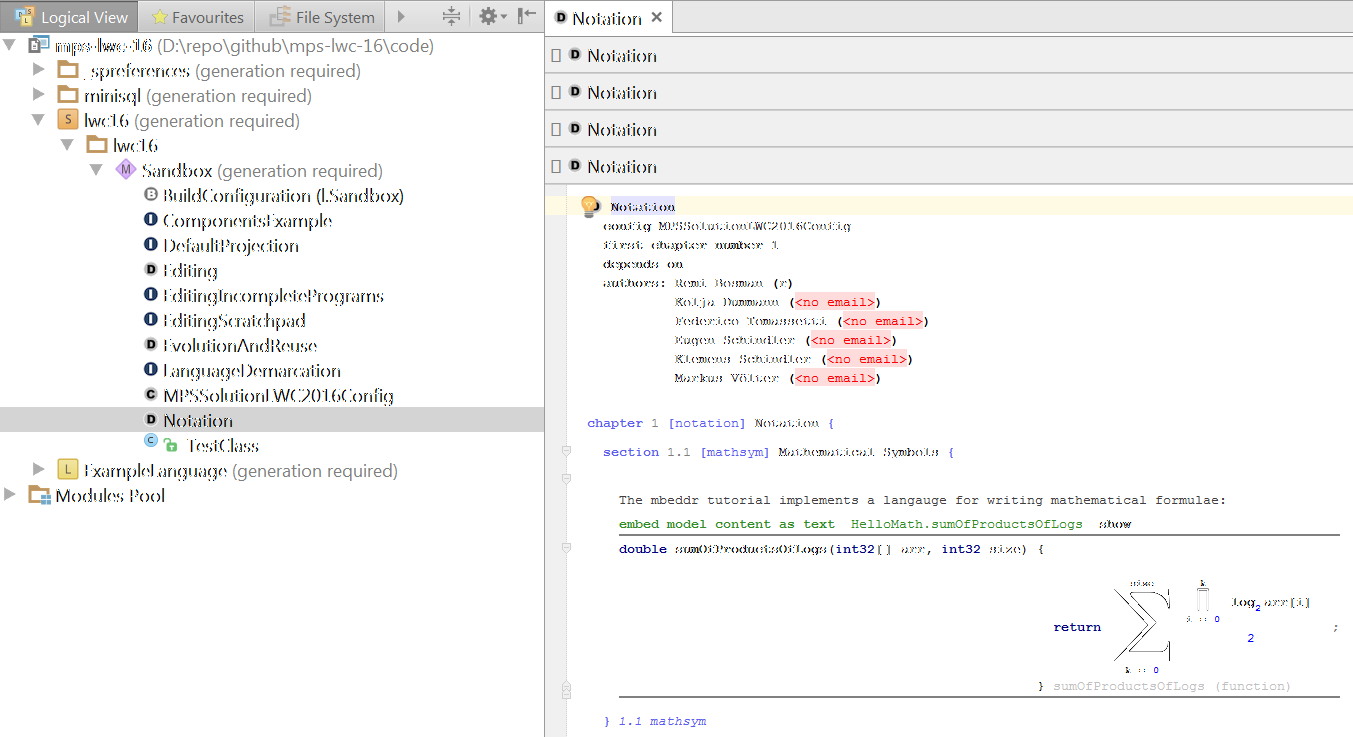
\includegraphics[width=0.50\textwidth]{screens/OpenNotation.png}
	\caption{The documentation model for the Notation challenge}
	\label{fig:opennotation}
\end{figure}

\subsection{Structure of the paper}

In the rest of the paper we present our proposed solutions to the
three different challenges (\emph{Notation, Evolution and Reuse, and Editing}).
For each challenge we start by describing the assumptions, then we
discuss the implementation, separately for each point, and finally we
analyze each challenge according to the schema suggested in the challenge
paper\cite{erdweg2015evaluating}:
Variants, Usability, Impact, Composability, Limitations, Uses and examples, Effort (best-effort), Other
comments, Artifact.
Finally, we will reflect back on the three challenges in the conclusions.

%%%%%%%%%%%%%%%%%%%%%%%%%%%%%%%%%%%%%%%%%%%%%%%%%%%%%%%%%%%%%%%%%%%%%%%%%%%%%%%
%
% Notation Section
%
%%%%%%%%%%%%%%%%%%%%%%%%%%%%%%%%%%%%%%%%%%%%%%%%%%%%%%%%%%%%%%%%%%%%%%%%%%%%%%%

\section{Addressing the Notation Problem}
The notation part of MPS is arguably one of its most powerful features.
That is so, because almost any notation can be rendered in an editor, from textual,
tabular and graphical to a mixture of these. Moreover, one can
define an arbitrary UI component as a cell in the editor (the editor in MPS is made
of cells\footnote{\url{https://confluence.jetbrains.com/display/MPSD31/Editor}}).

On the other hand, writing textual notations seamlessly requires more effort
from the language designer because of the projectional nature of MPS.
The classical example of writing a sum of two numbers in the editor by first writing the left-hand side
number followed by the plus sign and the right-hand side number requires additional
functions to be implemented in MPS.

\subsection{Assumptions}
We do not make any assumptions for the examples in the next sections. Notations and capabilities such as those
described next can be provided for any MPS languages.

\subsection{Implementation}
In the next subsections we present the chosen examples and the implementation for each
item of the \emph{Notation} challenge.

\subsubsection{Support mathematical symbols in addition to textual notation}
Figure \ref{fig:mathnotation} shows a mathematical calculation expressed in the mbeddr math language, which is embedded in a function of the mbeddr C language.
\begin{figure}[H]
	\centering
	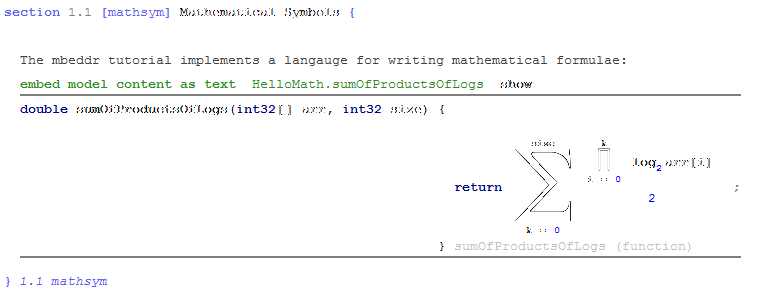
\includegraphics[width=0.50\textwidth]{screens/MathematicalNotation.png}
	\caption{Mathematical notation for the mbeddr math language}
	\label{fig:mathnotation}
\end{figure}

This notation is possible in MPS because one can insert any drawing in an editor cell using base language code (which is a reimplementation of Java).
The sum symbol, for instance, is placed in the editor component of the \emph{SumExpression} concept,
and the sum symbol is drawn on the screen using a \emph{Graphics} object in Java. Two screenshots from
the editor component of the \emph{SumExpression} concept and the implementation of the sum symbol
are shown in Figure \ref{fig:MathSymbolImpl}.

\begin{figure}[H]
	\centering
	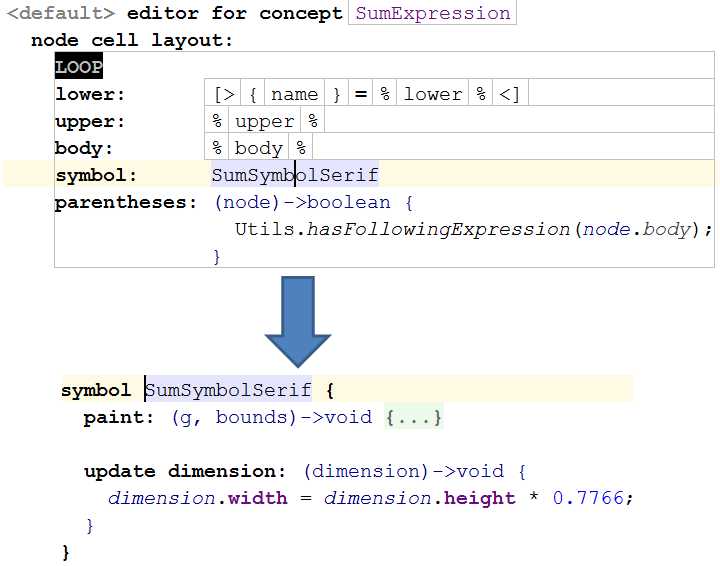
\includegraphics[width=0.45\textwidth]{screens/MathSymbolImpl.png}
	\caption{Editor component of the sum expression in the math language and the implementation
of the sum symbol with some details folded}
	\label{fig:MathSymbolImpl}
\end{figure}

\subsubsection{Support tabular notation in addition to textual notation}\label{sec:tabnot}
\begin{figure}[H]
	\centering
	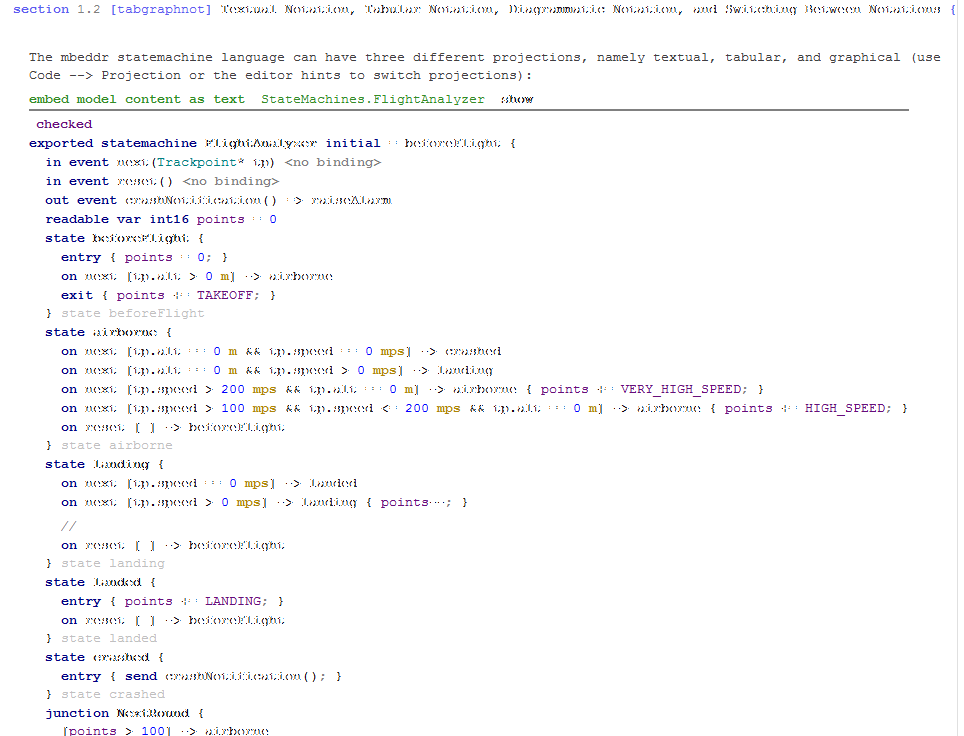
\includegraphics[width=0.45\textwidth]{screens/TextualNotationStatemachine.png}
	\caption{Textual notation for the mbeddr statemachine language with some details folded}
	\label{fig:txtnotationsm}
\end{figure}
\begin{figure}[H]
	\centering
	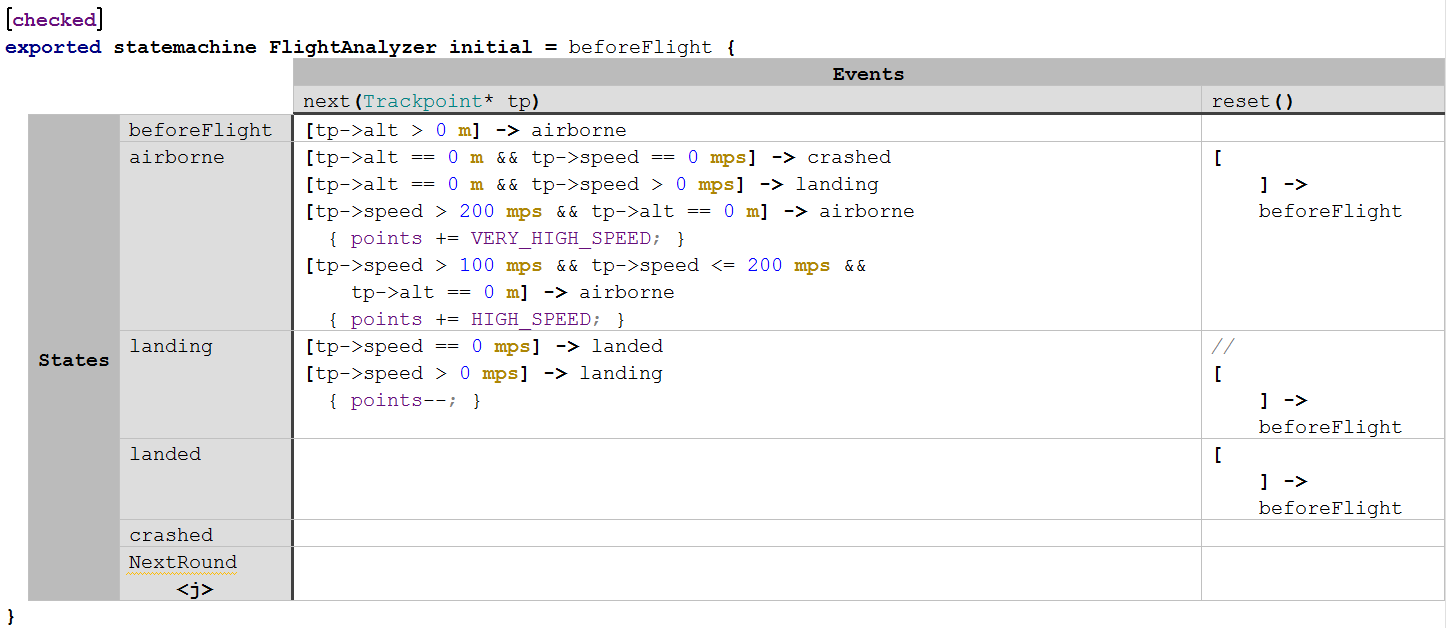
\includegraphics[width=0.50\textwidth]{screens/TabularNotationStatemachines.png}
	\caption{Tabular notation for the mbeddr statemachine language}
	\label{fig:tabnotationsm}
\end{figure}
Figure \ref{fig:txtnotationsm} shows a textual notation for the mbeddr statemachine language,
while Figure \ref{fig:tabnotationsm} shows a tabular notation for the same model expressed in the same statemachine language.

There can be multiple projections associated to models of a language because MPS permits an arbitrary
number of editors to be defined for the same language.
For instance, the tabular notation for the \emph{Statemachine} concept is defined
in a separate editor component where the columns, rows and cells of the concept are filled in
with the adequate properties, children and references of the \emph{Statemachine} concept.
An excerpt from this editor can be seen in Figure~\ref{fig:TableEditorStatemachine}.

\begin{figure}[H]
	\centering
	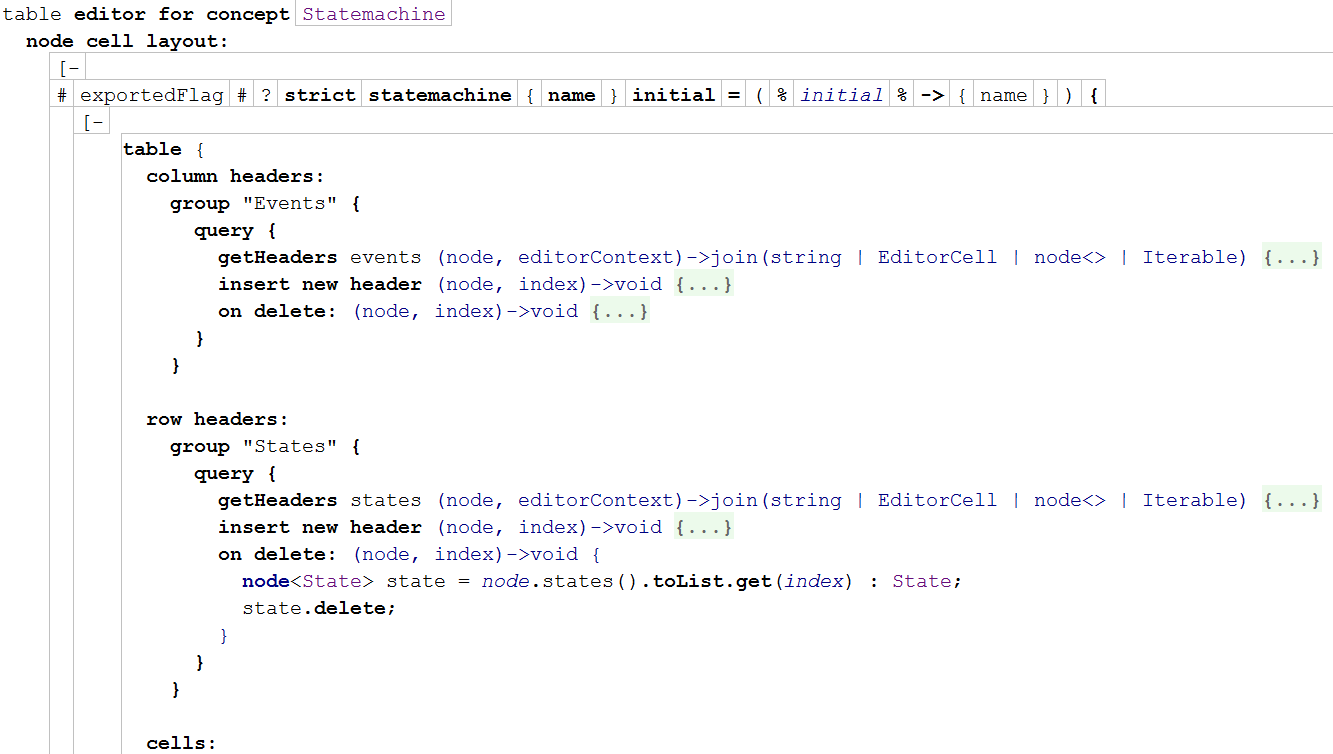
\includegraphics[width=0.50\textwidth]{screens/TableEditorStatemachine.png}
	\caption{Excerpt from the table editor for the \emph{Statemachine} concept with some details folded}
	\label{fig:TableEditorStatemachine}
\end{figure}

\subsubsection{Support diagrammatic notation in addition to textual notation}\label{sec:dianot}
\begin{figure}[H]
	\centering
	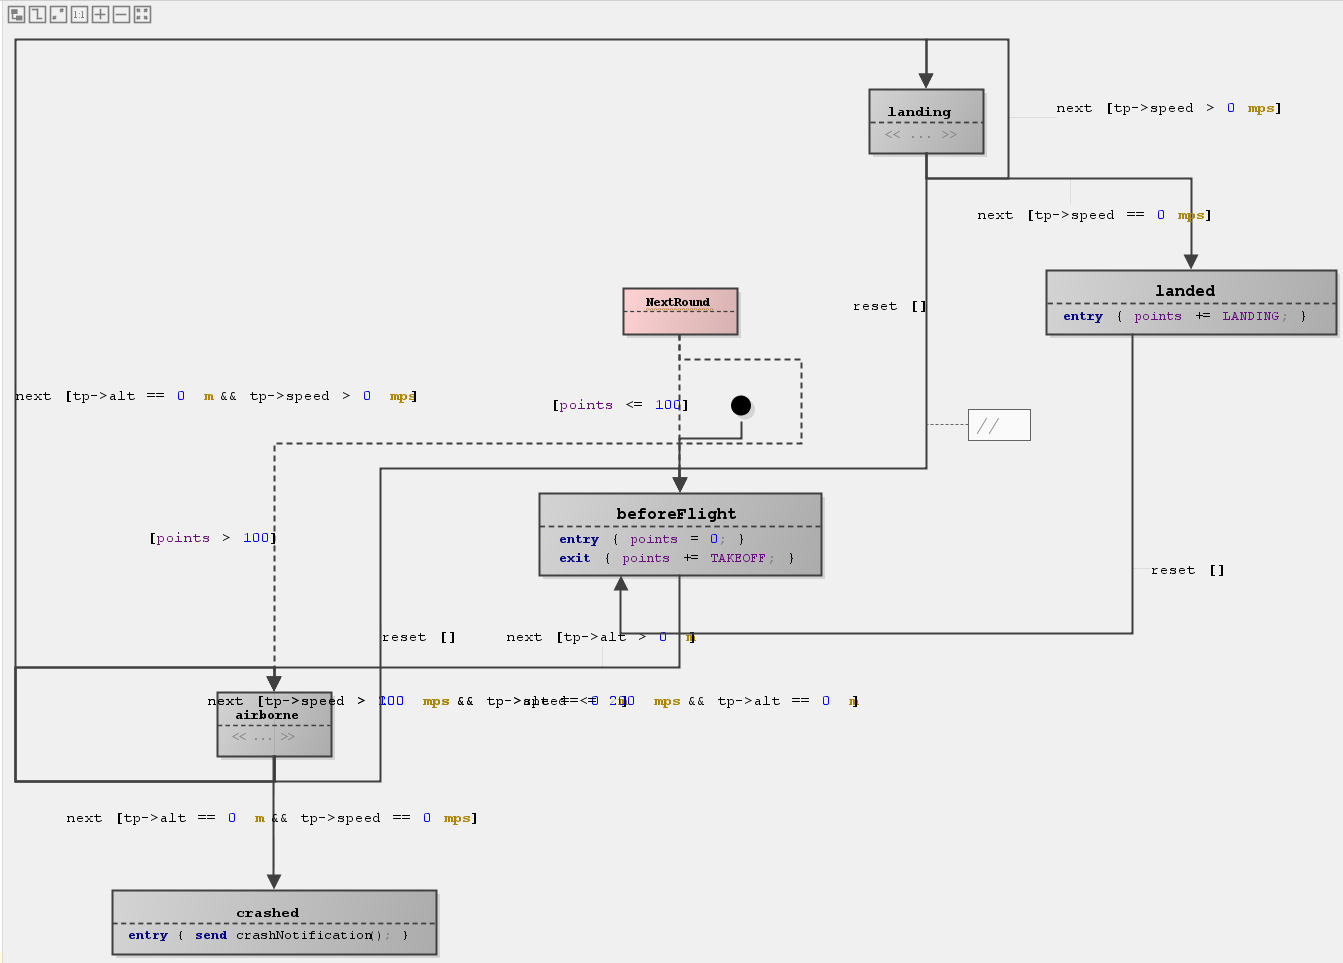
\includegraphics[width=0.50\textwidth]{screens/DiagrammaticNotationStatemachines.png}
	\caption{Diagrammatic notation for the mbeddr statemachine
	language}
	\label{fig:dianotationsm}
\end{figure}

Figure \ref{fig:dianotationsm} shows a diagrammatic notation for the mbeddr statemachine language for the same model from Section \ref{sec:tabnot}.
The diagrammatic notation for the \emph{Statemachine} concept is implemented in the same manner as described in the previous section,
by means of an editor component where the nodes and the edges of the \emph{Statemachine} concept
are filled in with the appropriate properties, children and references of the \emph{Statemachine} concept.

\subsubsection{Support switching between multiple alternative notations for the same language}
As shown in Sections \ref{sec:tabnot} and \ref{sec:dianot}, the notation for the same model written
in the mbeddr statemachine language can be alternated between textual, tabular, and diagrammatic.
MPS provides support for switching between alternative notations by means of so-called context hints.
A context hint is defined for each new editor provided for a language.
All the context hints defined for a language are added to a list that can be accessed from the viewer.
The context hints defined for the mbeddr statemachine language are shown in Figure~\ref{fig:contextHints}.

\begin{figure}[H]
	\centering
	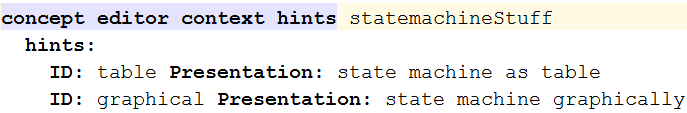
\includegraphics[width=0.50\textwidth]{screens/ContextHints.png}
	\caption{Context hints for the mbeddr statemachine language}
	\label{fig:contextHints}
\end{figure}

\subsubsection{Generic metadata annotations: annotation of program elements without changing their core meaning}
Annotations are called attributes in Jetbrain MPS.
For defining attributes of nodes in MPS, there exists the \emph{NodeAttribute} concept that can be attached
to almost any model node by default. Thus, when declaring generic metadata annotations, one needs to extend the \emph{NodeAttribute}
concept and define its contents. An example can be seen in Figure~\ref{fig:GenericNote} where a \emph{GenericNote} concept is defined.
To use the annotation, the language needs to be imported in the solution, and then, the \emph{GenericNote} concept can be attached to any
model node. For example, we have attached a generic note to both a paragraph in the documentation model and
a Java method, as can be seen in Figure~\ref{fig:exampleGenericNote}.

\begin{figure}[H]
	\centering
	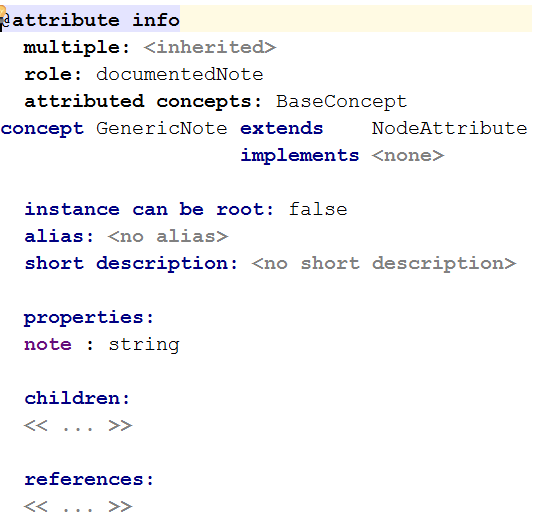
\includegraphics[width=0.50\textwidth]{screens/GenericNoteImpl.png}
	\caption{Structure of the generic note concept}
	\label{fig:GenericNote}
\end{figure}

\begin{figure}[H]
	\centering
	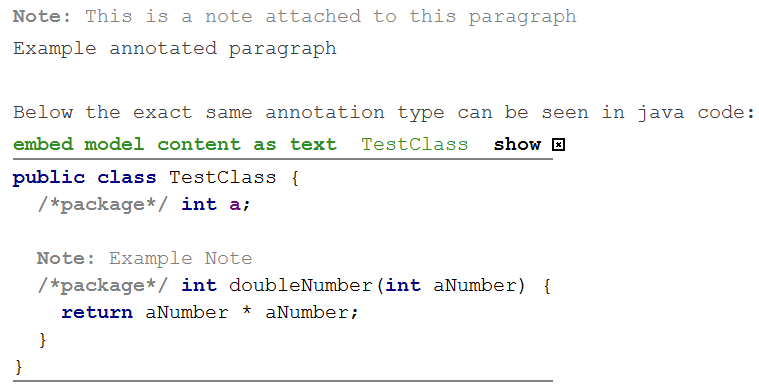
\includegraphics[width=0.45\textwidth]{screens/ExampleGenericNote.png}
	\caption{Two example uses of the generic note in the documentation model from github}
	\label{fig:exampleGenericNote}
\end{figure}

The metadata annotations do not change the model elements to which they are attached at all.

\subsubsection{Optional hiding: hide parts of the code, without losing the content and while retaining editability}
\label{sec:OptHiding}
The mbeddr environment supports product line variability \cite{voelter2015using}. In the variability language, users can define
feature models (see Figure~\ref{fig:featureModel}) and
different configurations of such features (see~Figure \ref{fig:configs}).
In the implementation code that makes use of the features of a feature model, presence conditions guard
code fragments (see Figure~\ref{fig:presenceCond}). A presence condition is a condition on features from the feature model.
Once a configuration is chosen, the code that is guarded with presence conditions that do not hold is taken out by the generator.
For more information on the feature models in mbeddr see Voelter et. al. \cite{voelter2013mbeddr}.

\begin{figure}[H]
	\centering
	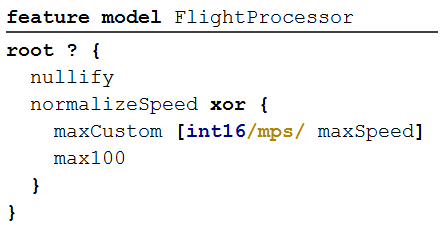
\includegraphics[width=0.30\textwidth]{screens/FeatureModelFlightProcessor.png}
	\caption{The feature model for flight processor}
	\label{fig:featureModel}
\end{figure}

\begin{figure}[H]
	\centering
	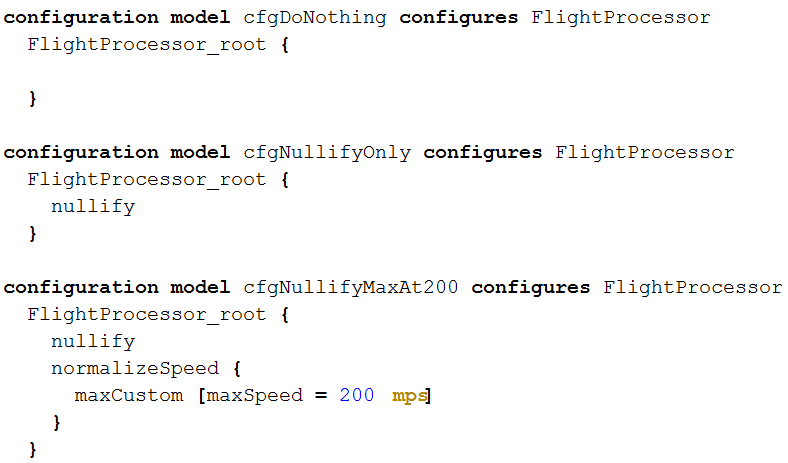
\includegraphics[width=0.50\textwidth]{screens/ConfigurationModels}
	\caption{Three configuration models given the feature model of the flight processor in Figure~\ref{fig:featureModel}}
	\label{fig:configs}
\end{figure}

\begin{figure}[H]
	\centering
	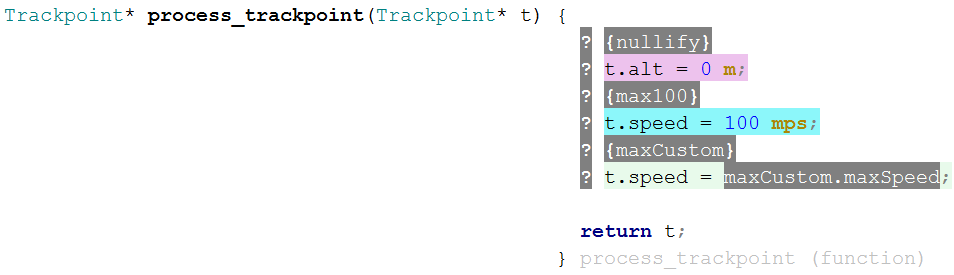
\includegraphics[width=0.50\textwidth]{screens/process_trackpoint.png}
	\caption{Function initializing a trackpoint by making use of presence conditions for elements from the
feature model in Figure~\ref{fig:featureModel}}
	\label{fig:presenceCond}
\end{figure}

The hiding of parts of the code is handled in the editor with the help of the \emph{show if} option.
Cells of the editor are conditioned by the \emph{show if} option. For instance, once a variant configuration has been chosen,
the editor can be updated to show the model with the processed presence conditions. Figure~\ref{fig:presenceConditionEditor}
illustrates how the viewing of the presence conditions are conditioned by a mode that is different from the compact mode.
Moreover, the changes to the viewer once the mode is changed via a menu action can be seen in Figure~\ref{fig:processTrackpointSelectedVariant}.

\begin{figure}[H]
	\centering
	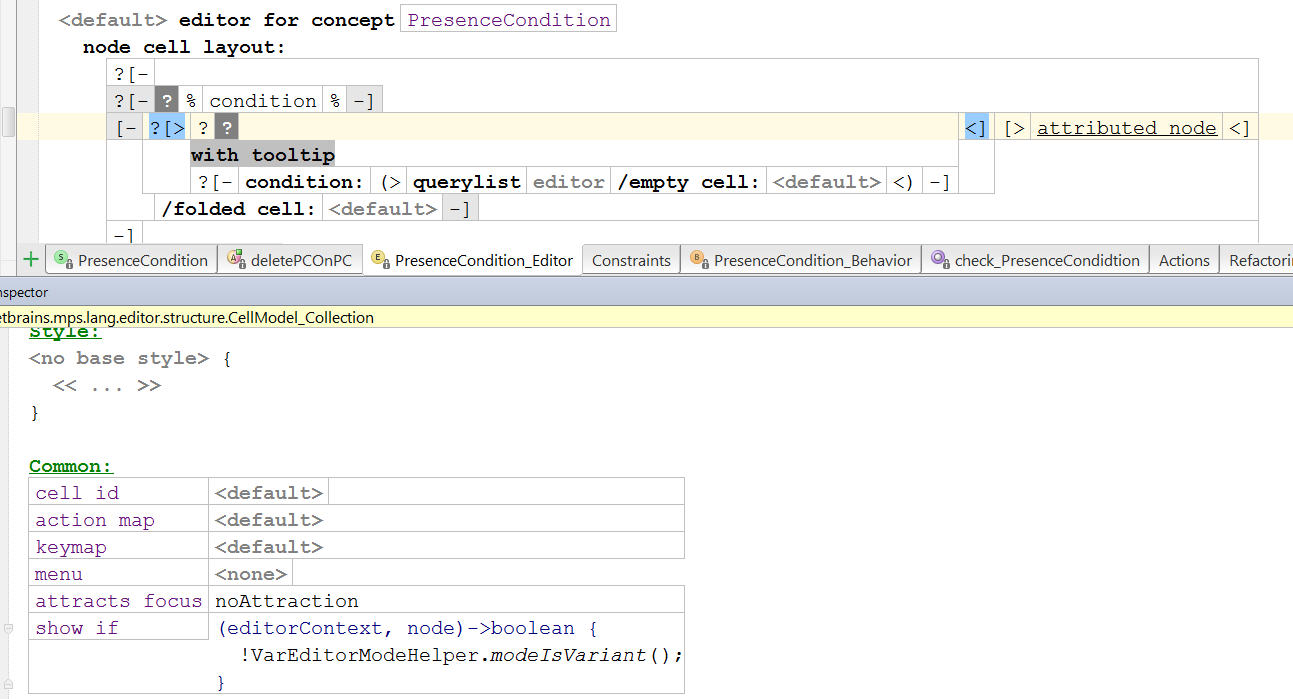
\includegraphics[width=0.50\textwidth]{screens/PresenceConditionEditor.png}
	\caption{The editor for concept \emph{PresenceCondition}}
	\label{fig:presenceConditionEditor}
\end{figure}

\begin{figure}[H]
	\centering
	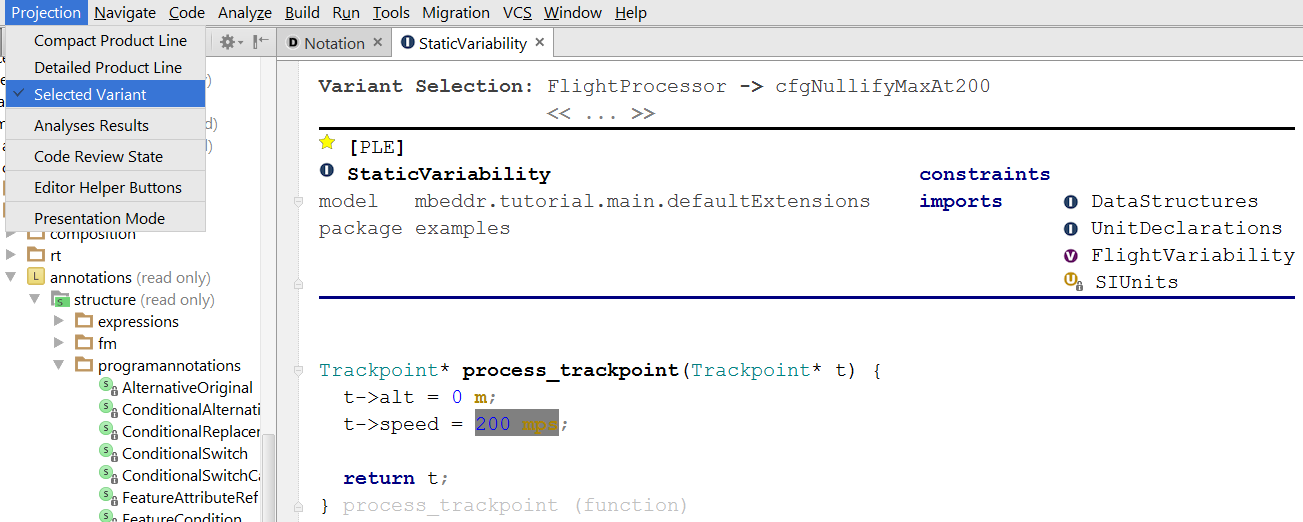
\includegraphics[width=0.50\textwidth]{screens/ProcessTrackpointSelectedVariant.png}
	\caption{The \emph{process\_trackpoint} function after changing the editor mode to the selected
variant}
	\label{fig:processTrackpointSelectedVariant}
\end{figure}
\subsubsection{Computed properties: read only annotations that are automatically derived form the main program}
The assert statements in mbeddr have an id that is read-only and that is derived from the main program. The number of the
id depends on the location of the assert statement in the main program. It is used mainly in logs  to
easily identify failed assert statements. An example of assert statements and their ids is given in Figure \ref{fig:asserts}.

\begin{figure}[H]
	\centering
	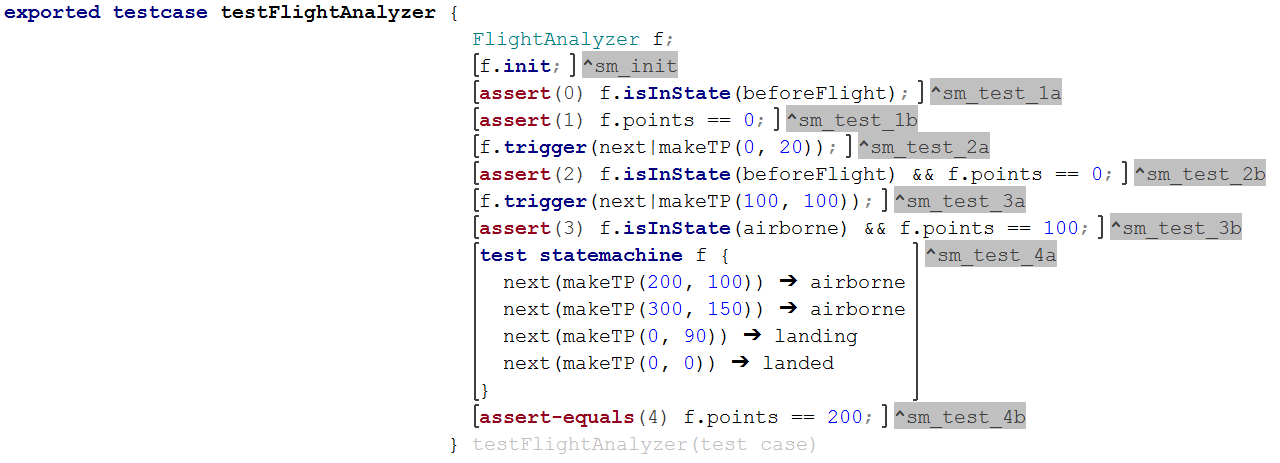
\includegraphics[width=0.50\textwidth]{screens/testFlightAnalyzer.png}
	\caption{Assert statements and their computed ids}
	\label{fig:asserts}
\end{figure}
\subsubsection{Computed structures: structured, editable views}
The signatures of mbeddr component operations are an example of computed structures.
Figure~\ref{fig:ComputedStructures} depicts component \emph{B}, which provides a port \emph{a} that refers to interface \emph{A}.
In this component, we create a runnable (component method) with an initial dummy name, \emph{aFloat}. We want this
runnable to be triggered by operation \emph{a.f} from the port \emph{a}.
When you execute the \emph{Synchronize} intention on \emph{aFloat}, it will get the same arguments as \emph{a.f}
automatically and its name will be updated consistently to \emph{portName\_methodName}.

\begin{figure}[H]
	\centering
	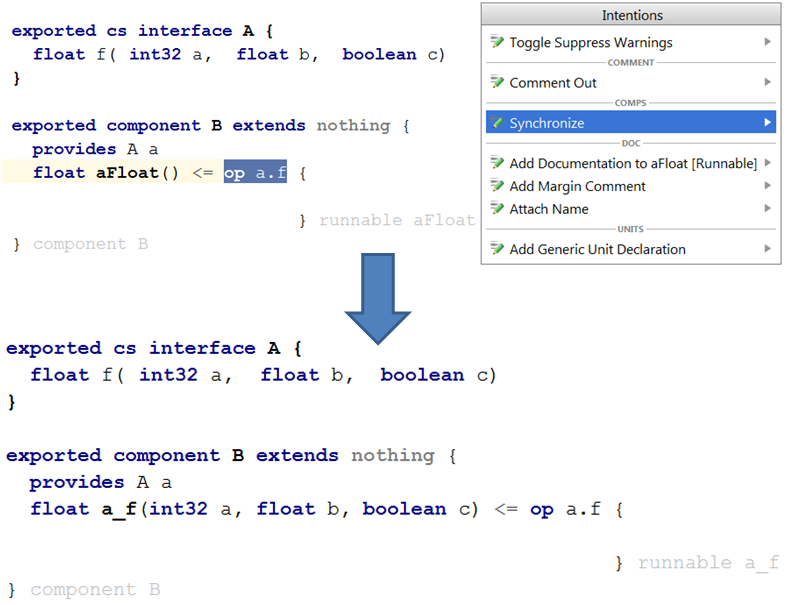
\includegraphics[width=0.50\textwidth]{screens/ComputedStructures.png}
	\caption{The synchronize intention automatically updates the runnable name and arguments.}
	\label{fig:ComputedStructures}
\end{figure}

The implementation of the synchronize intention is straightforward. Figure~\ref{fig:synchronizeRunnable}
depicts the implementation of the intention. The intention is defined for \emph{RunnableTrigger} concepts
and it calls method \emph{synchronizeRunnableParent} from concept \emph{RunnableTrigger}. The \emph{OperationTrigger}
is a sub-concept of \emph{RunnableTrigger} and it overrides method \emph{synchronizeRunnableParent}. The implementation
of the method is straightforward again, simply renaming the method name and adding the right arguments.

\begin{figure}[H]
	\centering
	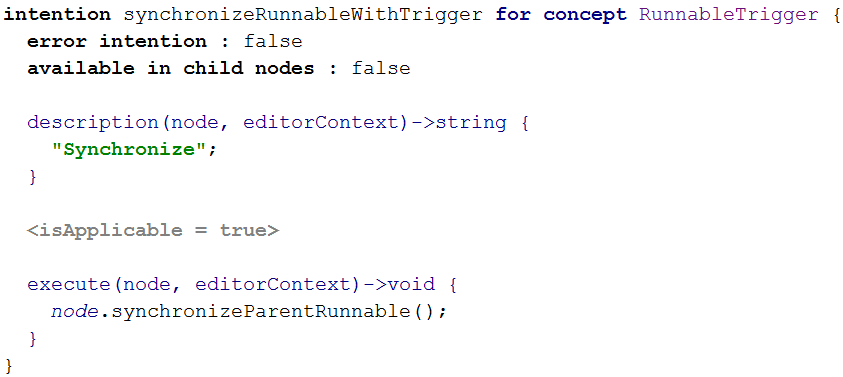
\includegraphics[width=0.50\textwidth]{screens/synchronizeRunnableWithTrigger.png}
	\caption{The implementation of the synchronize intention.}
	\label{fig:synchronizeRunnable}
\end{figure}
\subsubsection{Skeleton editing: guide the user with syntactic templates with editable holes}
The mbeddr build language is an example of a bigger structure with skeletons that can be edited.
The user makes a build configuration and some course-grained choices for the build (\emph{gcc}, \emph{microcontroller}, \emph{custom}, etc.),
and then she has a skeleton in which the details can be filled in. An example of a build configuration is shown in Figure~\ref{fig:buildConfigExample}.

\begin{figure}[H]
	\centering
	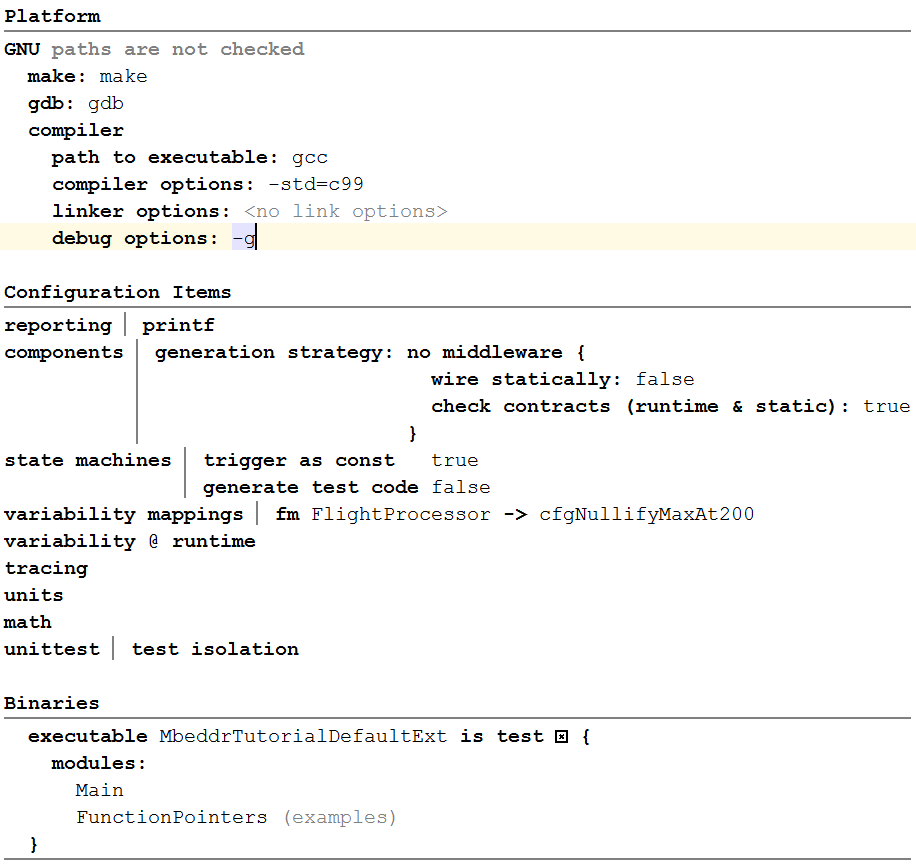
\includegraphics[width=0.50\textwidth]{screens/BuildConfigExample.png}
	\caption{A build configuration example.}
	\label{fig:buildConfigExample}
\end{figure}

Obtaining such a skeleton is possible through the editor aspect of a language. In this particular case,
in the editor for the build configuration language (see Figure~\ref{fig:buildConfigEditor}), there are three
sections specified: the platform, the configuration items and the binaries. The headers of these sections
are constant cells in the editor, and their constituent elements can be filled in by the user once the
build configuration is instantiated.

\begin{figure}[H]
	\centering
	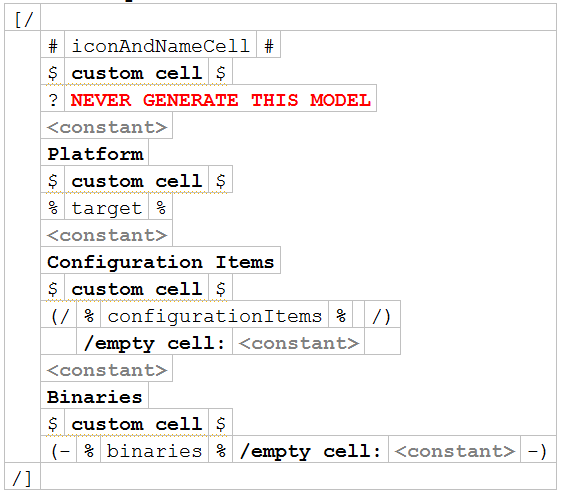
\includegraphics[width=0.50\textwidth]{screens/BuildConfigurationEditor.png}
	\caption{The editor for build configurations.}
	\label{fig:buildConfigEditor}
\end{figure}
\subsubsection{Embedding code in prose: mix structured code with free text}
One of the most relevant examples of code embedding in prose is the documentation language in mbeddr.
An example can be seen in Figure~\ref{fig:CodeInProse}. The figure shows an excerpt from the file
that was used to document and implement the language workbench competition's requirements of this year.

\begin{figure}[H]
	\centering
	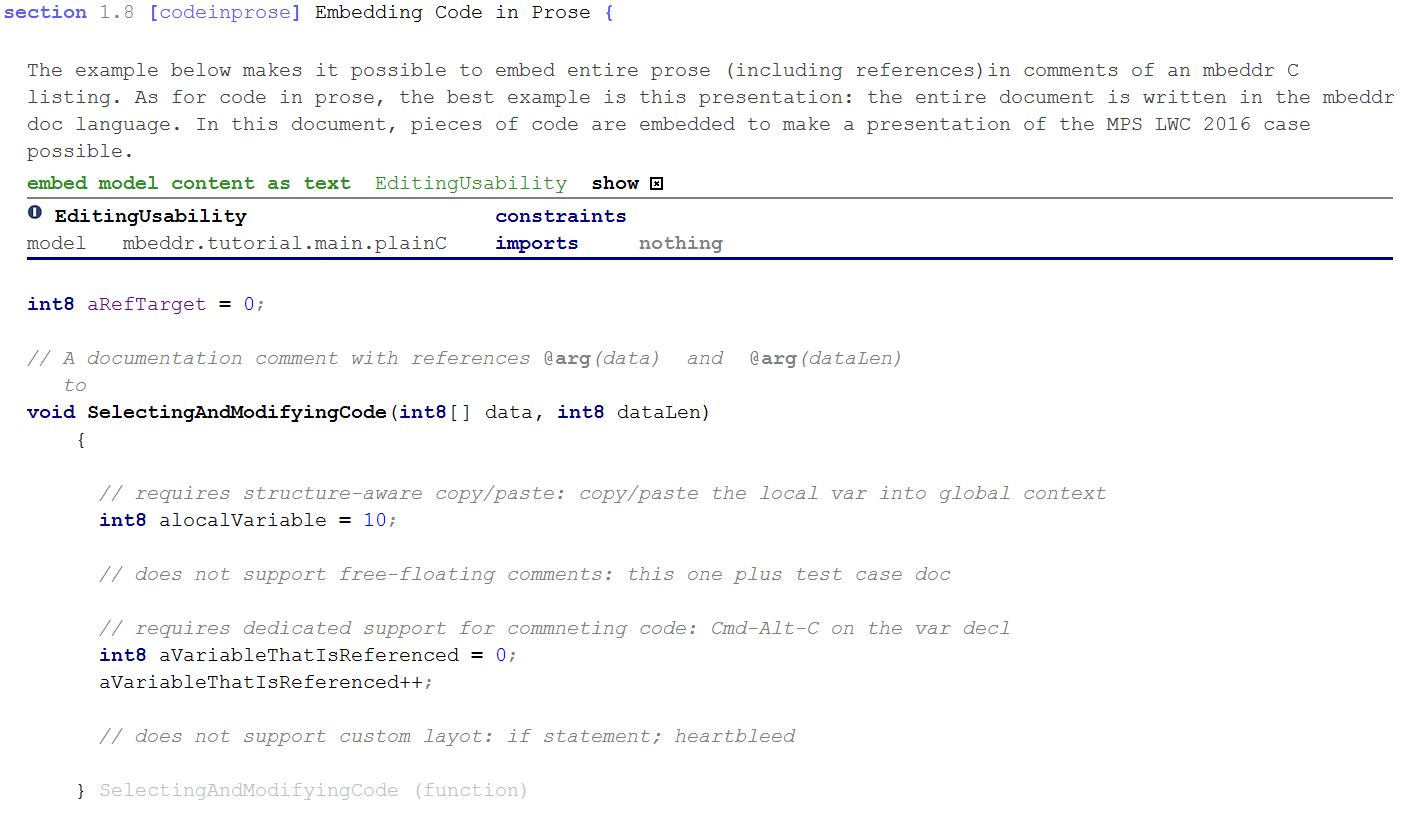
\includegraphics[width=0.50\textwidth]{screens/CodeInProse.png}
	\caption{Mixing prose and code.}
	\label{fig:CodeInProse}
\end{figure}

The documentation language has as a top-level concept the \emph{Document} concept. The document is formed of chapters. In turn, a chapter
is formed of sections and sections are formed of paragraphs. There are multiple types of paragraphs allowed in
the documentation language. One of them is \emph{ModelContentAsTextParagraph}. This type of paragraph
extends \emph{AbstractModelContentParagraph}, which contains model code pointers. Furthermore, a model code pointer contains
a collection of elements that can reference any named concepts in MPS (a named element implements interface
\emph{INamedConcept}). The referenced nodes are then embedded in the editor component.
Thus, \emph{ModelContentAsTextParagraph} can embed any piece of code that has a name property.
That allows us to embed an \emph{ImplementationModule}, for instance, as can be seen in Figure~\ref{fig:CodeInProse}.

Moreover, the text itself can contain actual references to concepts that are defined in mbeddr files.
This is achieved with the help of the \emph{mps-multiline} language, the \emph{mps-richtext} language
and the \emph{IWord} interface \cite{voelter2013integrating}.
If one has a concept that needs to be referenced from text (from comments or in the documentation language, for instance), then
that concept needs to implement the \emph{IWord} interface that simply presupposes to provide a string representation
for the concept. An example can be seen in Figure~\ref{fig:CodeInProse}, where the arguments of function
\emph{SelectingAndModifyingCode}, \emph{data} and \emph{dataLen}, are referenced from the comment attached
to the function.

Thus, in mbeddr, one can embed both code in prose and prose in code, giving rise to a mix of the two.
\subsubsection{Embedding blackboxes: allow program elements to be opaque non-textual elements}
We highlight the feature on embedding blackboxes in MPS with the embedding of images
in the documentation language. An example of an image introduced in a document in mbeddr is shown in Figure~\ref{fig:ImageInDoc}.

\begin{figure}[H]
	\centering
	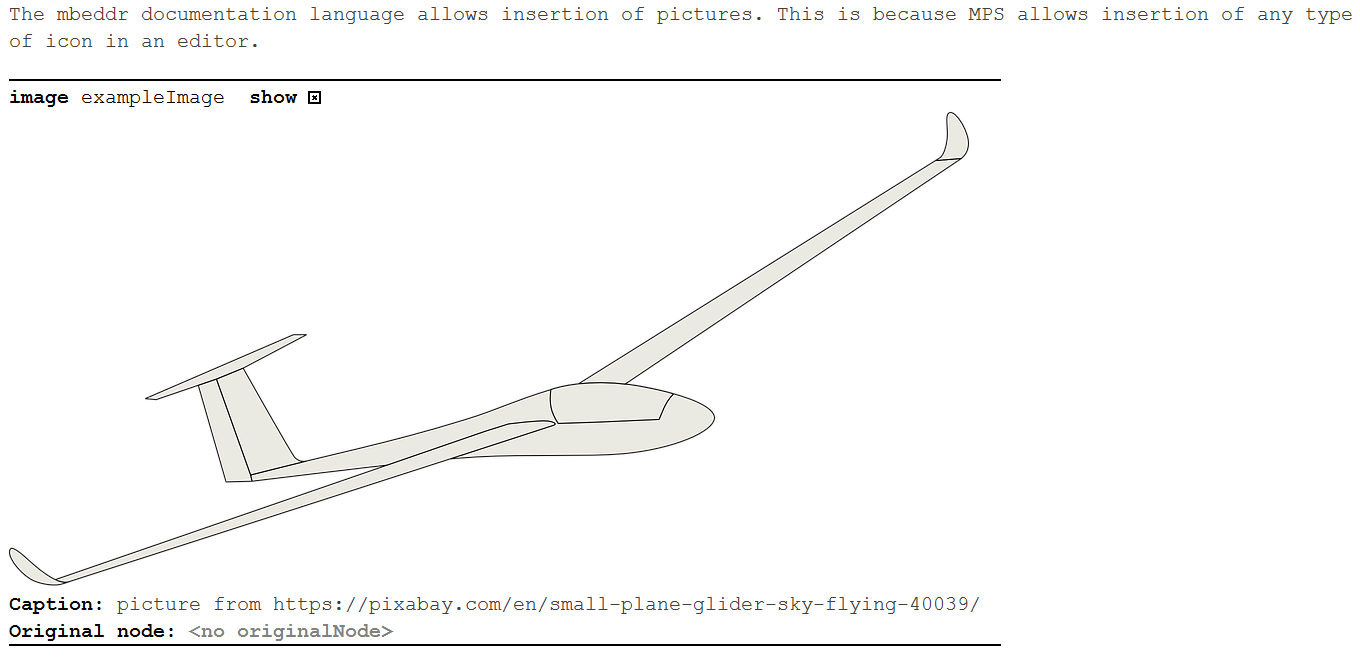
\includegraphics[width=0.50\textwidth]{screens/PlaneGlider.png}
	\caption{Embedding of an image into an mbeddr documentation file.}
	\label{fig:ImageInDoc}
\end{figure}

As discussed in the previous section, the \emph{Document} concept is ultimately formed of paragraphs.
In the mbeddr documentation language, one type of paragraph is the \emph{ImageParagraph}. The editor
component of \emph{ImageParagraph} embeds a swing component, and this specifies how to render an image
with a given path. Part of the implementation can be seen in Figure~\ref{fig:EditorImageParagraph}.
Now, once a valid image path is specified in the document, the respective image
is rendered in the editor. The image itself is a blackbox from the point of view of the document.

\begin{figure}[H]
	\centering
	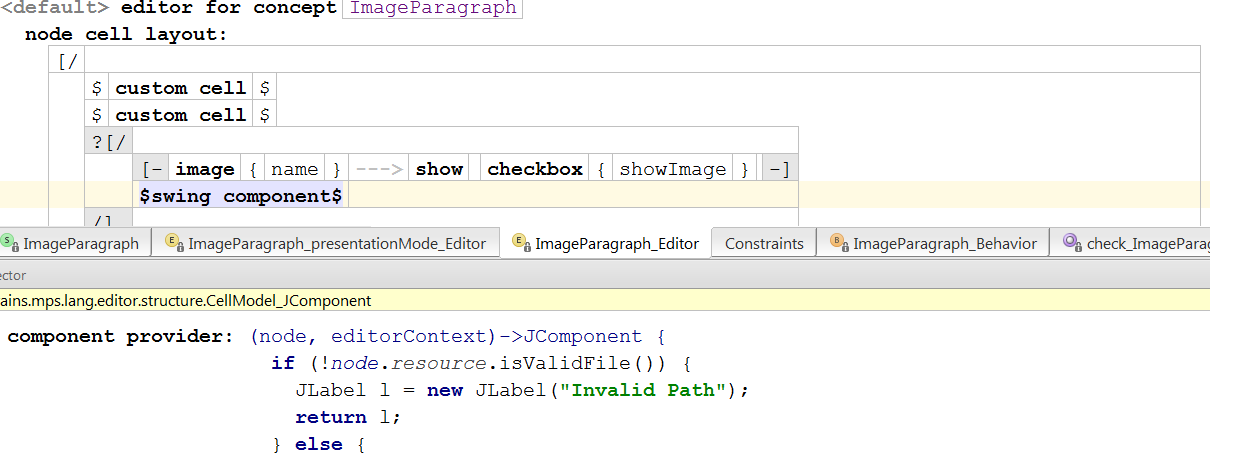
\includegraphics[width=0.50\textwidth]{screens/EditorImageParagraph.png}
	\caption{Part of the implementation of a swing component in the editor of concept \emph{ImageParagraph}.}
	\label{fig:EditorImageParagraph}
\end{figure}

\subsection{Variants}
There were other alternatives for showcasing some of the features presented in the previous sections.
We will give here a few variants only.

Switching between notations can be accomplished not only through context hints, but with
different user actions as well. In the state machine language, one can switch between different
projections by using the \emph{Projection} tab and selecting the desired projection. Details on this
can be found in our documentation model on github, in the \emph{Notation} section. In the implementation in mbeddr,
there is a plugin that introduces this tab and that triggers the projection selected.

There are also many other examples for the optional hiding feature. Some characteristics of concepts
can be hidden and toggled with an intention, for instance. Take the export statement for modules as an example, which can
be tried on modules in the documentation model on github. The intention toggles the value of the boolean property \emph{exported},
which results in showing/hiding the export statement depending on the condition expressed in the editor of the concept
(similar to the discussion in Section~\ref{sec:OptHiding}).

One other variant that can be used as an example to showcase the power of MPS
is the notation in the form of a PlantUML\footnote{\url{http://plantuml.com/}} diagram of the
state machine languages. MPS allows to incorporate viewers in the editor that project a model in a language
written in MPS.

\subsection{Usability}
The effort to make the notations as usable as possible goes to the language designer. The drawbacks of the
projectional editors are well-known, but MPS goes a long way to provide tools to the language
designer that help in creating a user-friendly editor \cite{voelter2014towards}.
The notations provided in mbeddr are a good example of user-friendly notations.

\subsection{Impact}
Introducing notations to a language does not come with a big negative impact on the language.
The notation is expressed in an editor aspect, that is provided for each concept, and this aspect
does not usually influence the other aspects of the language.
At most, the editor aspect might require the import of certain libraries, and that has an impact on the overall
language because the import is going to be added to the dependency list of the language itself.

There are situations when the impact of the notation can be considerable on the language. If one uses the default
graphical notation provided by MPS (instead of the graphical notation provided in mbeddr), one might need to
change the structure of the language itself. This has a very big impact, because all the other aspects of the language
depend on the structure. The changes are required if the elements that need to be represented as edges in the graphical representation
are not concepts in the language itself. That would mean transforming those elements into concepts first.

\subsection{Composability}
Each concept in a language can have any number of editors attached to it. The different editors of a concept $C$
do not interact among each others, unless one editor of $C$ reuses another editor of $C$ (reuse of editors for the same concept
is possible in MPS). One common pattern is to define an editor component for an interface concept and reuse that
editor component in the editor of a concept that implements the interface concept. This can be noticed in the
mbeddr code with concept \emph{StateMachine} and interface concept \emph{IModuleContent}, for instance.

Composability is very well supported at the editor level, because each editor is made of cells,
and cells, in turn, are formed of other cells. This permits defining
the editor of a concept as a collection of cells, where some cells are the editors of the children of the concept.

Moreover, a sub-concept inherits the editor (the notations) of its super-concept. If this is not the desired behaviour,
the editors of the sub-concepts can be overriden as well.

\subsection{Limitations}
The notations introduced can be used only inside MPS. That applies also to the textual notations, because
the files are persisted as XML on disk, and they are projected as text on the screen.

Moreover, as already mentioned, there are certain limitations inherent to projectional editors especially
when it comes to textual notations, but this limitations are well mitigated by MPS \cite{voelter2014towards}.

\subsection{Uses and examples}
The uses and examples have been covered in the implementation section.
Almost all examples in that section are from mbeddr, with the exception of the generic metadata annotation,
where we created a separate language with the generic note concept. This language and the generic note concept
can be found on the github repository of our submission.

\subsection{Effort (best-effort)}
Some of the items described in the previous sections are trivial to address (in the order of a few minutes):
\begin{itemize}
\item The skeleton editing is provided by default in Jetbrains MPS and is a natural consequence
of how editors are created in Jetbrains MPS.
\item The switching between notations is a matter of introducing one context hint, that is one file and a name for the
context hint.
\item The optional hiding is a matter of writing one condition in the editor cell
that should be hidden.
\item Embedding code in prose is trivial if we want to make references to elements defined in code in text, because
it requires implementing one interface and defining one operation.
\item Computed structures and properties such as the one exemplified imply the implementation of a function that computes the
necessary structures.
\item Generic metadata annotations are trivial to add to model elements as well, because they involve only defining a new
concept that extends the node attribute.
\end{itemize}

Other items require more time (in the order of a few minutes to a few hours, depending on the size of the language):
\begin{itemize}
\item The tabular notation can be more involved because it requires that a few functions are provided
to fill in the columns and the rows of the table.
\item The same holds for the diagrammatic notation where code needs to be filled in that specifies what concepts
are going to fulfill the role of edges and nodes and under what conditions.
\item Embedding entire chunks of code in prose requires more effort than simply referencing an element from code in text.
\end{itemize}

More involved items that require considerable time (in the order of a few hours to a day):
\begin{itemize}
\item Embedding blackboxes, such as images, requires that one implements the logic to render the image in the
editor and the logic to read the path of such images.
\item Showing math symbols in the editor takes more time as well, as the rendering of the symbol in the viewer needs to be
implemented.
\end{itemize}

\subsection{Artifact}
The examples discussed about in this section can all be found in the documentation model in the \emph{Notation} section.
As for their implementation, that resides in the mbeddr code (see file \emph{README.md} for the version of mbeddr we used).

%%%%%%%%%%%%%%%%%%%%%%%%%%%%%%%%%%%%%%%%%%%%%%%%%%%%%%%%%%%%%%%%%%%%%%%%%%%%%%%
%
% Evolution and Reuse Section
%
%%%%%%%%%%%%%%%%%%%%%%%%%%%%%%%%%%%%%%%%%%%%%%%%%%%%%%%%%%%%%%%%%%%%%%%%%%%%%%%

\section{Addressing the Evolution and Reuse Problem}

In this section we present our solution to the challenge on Evolution and Reuse.

\subsection{Assumptions}

Our solutions are presented making references to the two main language families developed for MPS.

First of all we have the BaseLanguage, which is an implementation of Java built from JetBrains and shipped with MPS. Several extensions are distributed with MPS, including extensions to support lambdas, manipulation of sequences, expressions to access MPS concepts and models, etc.

Another very popular family of languages is mbeddr. It is an implementation of the C language in MPS with support for variability, state machines, testing, documentation and more. In addition to that, the mbeddr platform has been created. It is a collection of language extensions not specifically related to mbeddr or the C language. These extensions proved to be useful in different contexts.

\subsection{Implementation}

In this subsection we present how we implemented a solution to each specific challenge.

\subsubsection{Language extension: modularly extend a language with new syntactic constructs}
\label{evr:langext}

In this section, we are going to describe the mbeddr language for state
machines with event-driven execution. The mbeddr state machines extends
the base language from MPS. This enables a seamless integration between
C code and state machine specifications.

State machines are a mathematical model of computation often used in embedded software
for describing discrete behaviour through state transitions. Its characterizing
ingredients are states, transitions and events. At any given time, a state
machine is in a state and it can be transitioned from one state to another.
A transition in a state machine is triggered by an event. These events
are usually provided by the environment, and, hence, the state machine
needs to have a way to interact with the environment. Besides events,
transitions can also have different guard expressions that need to hold when
the event arrives, for the transitions to be triggered.

We are now going to describe the extension of mbeddr with new syntactic notations for state machines.

In mbeddr, the state machine language is packaged in a language module and it
extends the base language of MPS. The \emph{StateMachine} concept extends
\emph{BaseConcept}, which means that the state machine is a program node,
as \emph{BaseConcept} is the concept from which all other concepts are derived.
The state machine language also implements the \emph{IModuleContent} interface,
which means that they can be top-level components in modules or can be inside of any
container that expects \emph{IModuleContent} children. Modules in mbeddr C
introduce basic program modularization, visibility control and namespaces \cite{voelter2013mbeddr}.

In the next paragraphs, we are going to present excerpts from a state machine for
judging flights. The state machine awards points for successful
takeoff and landing and for speed flown \cite{voelter2014generic}.

The state machine adds custom notation for specifying the state machine. The textual
form of the state machine can be seen in Figure \ref{fig:HFAT}. The figure depicts a hierarchical state machine
that computes the points for a flight.
In addition, because textual forms can live alongside graphical and tabular forms in MPS,
the state machine can be viewed in table form and graphical form as well alongside the piece of C code
where it is used. Figure \ref{fig:HFATab} shows the same state machine for flight analyzes in tabular form.

\begin{figure}[H]
	\centering
	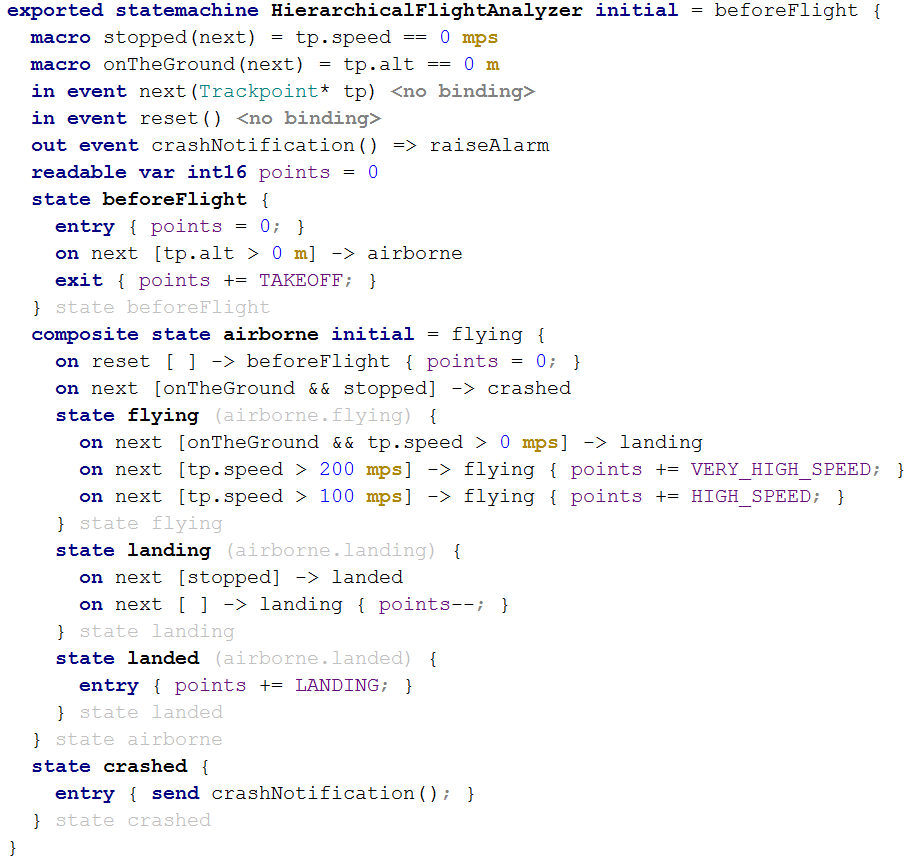
\includegraphics[scale=0.5]{screens/HierarchicalFlightAnalyzerT}
	\caption{Hierarchical flight analyzer state machine - textual notation}
	\label{fig:HFAT}
\end{figure}

\begin{figure*}[ht!]
	\centering
	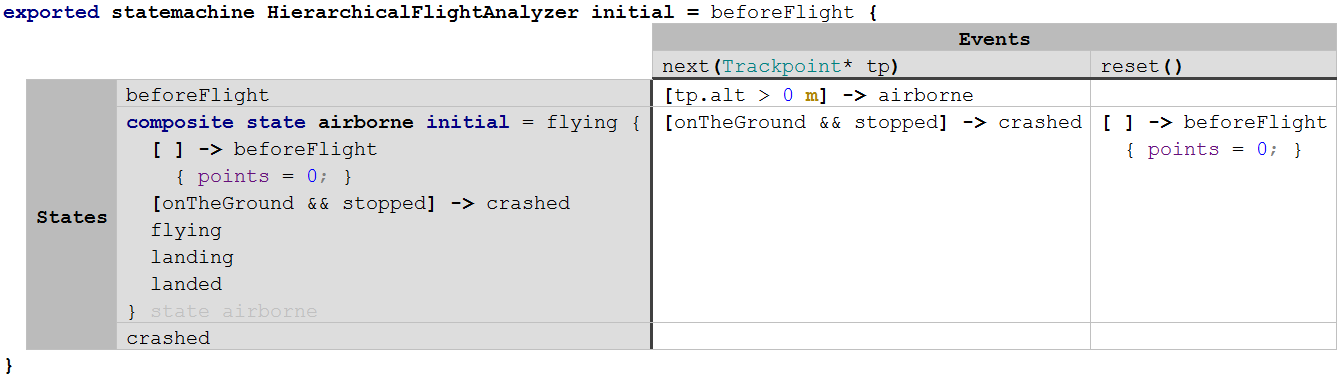
\includegraphics[scale=0.55]{screens/HierarchicalFlightAnalyzerTab}
	\caption{Hierarchical flight analyzer state machine - tabular notation}
	\label{fig:HFATab}
\end{figure*}

Moreover, the state machine itself embeds arbitrary code in the actions
and in the guards. The actions are statement lists and the guards are expressions.
For instance, look at the guards and actions in Figure \ref{fig:HFAT}; they contain mbeddr C expression.

\subsubsection{Language embedding: embed a separate language inside another}
\label{evr:langembed}

We have implemented a simple toy language representing a subset of SQL. This language permits to define database schemas and simple SQL statements referring to such schemas.

Typically SQL is used in combinations with General Purpose Languages (GPLs): from the GPLs queries are generated by filling SQL templates with variable elements. The results of these queries are then possibly processed using GPL code.

In our example we implemented both embedding of C code into our MiniSQL and embedding of MiniSQL into C.
By embedding C code in MiniSQL we can define SQL statements with variable elements. For example we can refer to a C variable containing an ID in our SQL statement. In this way we can vary the value of the variable to obtain parametric SQL queries. We can then execute those queries using libraries such as those based on ODBC\footnote{See \url{https://en.wikipedia.org/wiki/Open_Database_Connectivity}}. It is important to notice that the MiniSQL embedded in C can be still edited with proper support regarding validation and auto-completion. It is not \"just a string\".
This technique is illustrated in \ref{fig:sqlembedding}.

\begin{figure}[H]
	\centering
	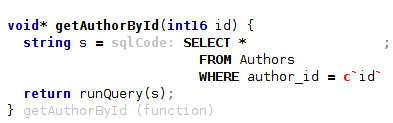
\includegraphics[width=0.50\textwidth]{screens/minisql_embedded.png}
	\caption{Embedding SQL code into C code and viceversa}
	\label{fig:sqlembedding}
\end{figure}

To demonstrate the flexibility of this approach we have also embedded our MiniSQL into the BaseLanguage, which is basically an implementation of Java in MPS. You can see it in \ref{fig:sqlembeddingjava}. Two separate extensions permit to embed the same language into different hosts (C and Java). For further explanations on this approach refer to \cite{Tomassetti2013}.

\begin{figure}[H]
	\centering
	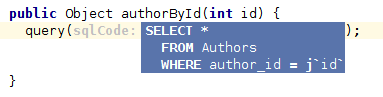
\includegraphics[width=0.50\textwidth]{screens/minisql_embedded_java.png}
	\caption{Embedding SQL code into Java code and viceversa}
	\label{fig:sqlembeddingjava}
\end{figure}

\subsubsection{Extension composition: combine independently developed extensions}
\label{evr:langcomp}

The mbeddr project contains many examples of language composition. Different extensions have been developed during the years, not necessarily from the exact same persons or in the context of the same project. However all of these extensions can be combined and used together.

A very interesting example is the Documentation language which permits to add references to other portions of code or to embed specificy contructs into the documentation.

In the example in \ref{fig:extensioncomposition} we can see a Documentation construct containing a table. The tables extensions have been developed separately, in a completely agnostic way, so that it could be reused in very different contexts. In this case it contains expressions from mbeddr language (C). So effectively three different extensions are combined in one single example.

\begin{figure}[H]
	\centering
	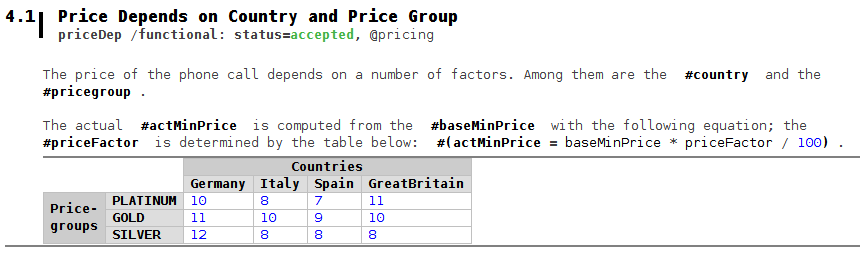
\includegraphics[width=0.50\textwidth]{screens/extension_composition.png}
	\caption{Combining tables, C expressions and the documentation language}
	\label{fig:extensioncomposition}
\end{figure}

\subsubsection{Beyond grammar restrictions: disallow constructs in certain scopes, without modeling this in the (abstract) syntax}
\label{evr:beyondgrammar}

MPS offers several mechanisms to limit where a certain construct can be used. In this respect it is not limited to the abstract syntax definition, but further logic can be added to additionally constraints the concepts usable in a given scope.

For example, every \emph{AssertStatement} is technically an mbeddr \emph{Statement}, from the point of the abstract syntax. However, an additional rule has been defined to restricted all constructs marked as \emph{IRestrictToTests} to be used exclusively in tests or tests related helper functions. This rule is visible in \ref{fig:restrictedtotest}.

\begin{figure}[H]
	\centering
	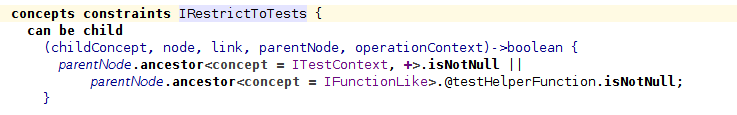
\includegraphics[width=0.50\textwidth]{screens/restricted_to_test.png}
	\caption{Rule which constraints the usage of certain constructs to tests}
	\label{fig:restrictedtotest}
\end{figure}

\subsubsection{Syntax migration: support migrating programs when concrete syntax changes}
\label{evr:synmigr}

\comment{TODO: to be written after the examples are provided}

\subsubsection{Structure migration: support migrating programs when abstract syntax changes}
\label{evr:structmigr}

\comment{TODO: to be written after the examples are provided}

\subsection{Variants}

The three first points we have seens (\ref{evr:langext}, \ref{evr:langembed}, and \ref{evr:langcomp}) have been solved through simple extension techniques. We do not see any obvious alternative for such cases. About combining independently defined extensions (\ref{evr:langcomp}) we can consider all the projects using the mbeddr platform as examples of this technique.

Regarding the grammar restrictions (\ref{evr:beyondgrammar}), we implemented it specifiying that certain rules can have as ancestors only certain nodes. Conversely we could have specified that certain rules could not contain specific descendants instead.

\subsection{Usability}

From the point of view of usability \ref{evr:langext}, \ref{evr:langembed}, and \ref{evr:langcomp} do not pose any issue. We simply used the mechanism of language extensions to add additional constructs to existing language. In one case we had done that for the specific goal to embed another language, while in the other cases we did not. In all cases the new constructs can be used exactly as the existing ones, so the new constructs are as usable as the previous ones with no different interactions required to the users.

The grammar restriction presented in \ref{evr:beyondgrammar} does not pose any usability issue neither. The whole mechanism is transparent to the user: elements which cannot be used in a certain context are not offered by the auto-completion mechanism and there is no immediate way to use them when they are not supposed to be used.

Migrations are typically performed through wizard dialogs. Those migrations are proposed to the user when MPS is started or the user can trigger them manually.

\subsection{Impact}

Language composition does not require to change existing elements.

\subsection{Composability}

Language composition is well supported in MPS. It is very natural and it does not require any particular technique. The only possible issues could be caused by semantic conflicts: suppose an expression language defines only statically evaluable expressions such as literals and basic mathematical expressions. Furthermore, suppose a first extension is based on this consideration and adds the possibility to display the result of such expressions. Now, if a second extension would introduce non-statically evaluable expressions, the two extensions would not interact well together. This problem could be avoided by planning for extensibility in the original language: for example we could have required each \emph{Expression} concept to declare if it was statically evaluable or not. All the expressions of the original language would have declared themselves to be statically evaluable, while the Expressions from the first extension would have not. The extensions calculating result values could have used the method to verify that all Expressions for which it wanted to calculate a value were indeed statically evaluable and trigger an error when not-statically evaluable expressions were used in the wrong context. In this way the two extensions would interact nicely without being aware of each other.

\subsection{Limitations}

No particular limitations come to mind.

The only limitation we see is with migrations, because they are not reversible. This is an issue when different members of a team want to use different versions of MPS because each version comes with specific versions of the BaseLanguage: when a project is open with a new version, migrations have to be performed and these migrations make the project incompatible with previous versions. Effectively this forces everyone to use the same version of the language workbench.

\subsection{Uses and examples}

Language extensibility and composition are used extensively in the two well-known MPS language families: the BaseLanguage and mbeddr. The BaseLanguage defines a core language and a set of independent extensions, mbeddr does the same.

\subsection{Effort (best-effort)}
\ana{Maybe it is easier to write this subsection in the same manner we have wrote about effort in the notation section.}
The estimated effort for the different points are:

\begin{itemize}
	\item Language extension: XXX minutes
	\item Language embedding: 10 minutes
	\item Extension composition:
	\item Beyong grammar restrictions:
	\item Syntax migration:
	\item Structure migration:
\end{itemize}

For \emph{Language embedding} we calculate only the time for creating the concepts wrapping constructs of one language to be used in the other one (SQL into C and C into SQL). This time considers the definitions of the concepts, the editors, the typesystem rules and the code generators.

\subsection{Other comments}

\comment{Any idea?}

\subsection{Artifact}

\comment{TODO understand what should we write in this section}
\ana{I assume that this refers to the actual artifacts that we created: the
examples in the documentation models and the mbeddr code itself}.

%%%%%%%%%%%%%%%%%%%%%%%%%%%%%%%%%%%%%%%%%%%%%%%%%%%%%%%%%%%%%%%%%%%%%%%%%%%%%%%
%
% Editing Section
%
%%%%%%%%%%%%%%%%%%%%%%%%%%%%%%%%%%%%%%%%%%%%%%%%%%%%%%%%%%%%%%%%%%%%%%%%%%%%%%%

\section{Addressing the Editing Problem}

\subsection{Assumptions}

\subsection{Implementation}

\subsubsection{Editing incomplete programs: support for syntactically malformed programs}
\begin{figure}[H]
	\centering
	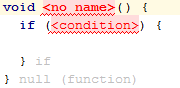
\includegraphics[width=0.25\textwidth]{screens/IncompleteNode.png}
	\caption{An incomplete function with missing name, containing an if statement missing a guard.}
	\label{fig:IncompleteNode}
\end{figure}

It is possible to edit and persist an incomplete model, however there are some restrictions to this. A node, for example an if statement, must have a complete skeleton. It is possible to leave content out such as the guard and body in an if statement. The result can be considered syntactically incorrect since the guard missing from if statement. However, the construction is still structurally sound since it is a valid tree node, albeit with some gaps to be filled in. Figure~\ref{fig:IncompleteNode} shows an example of a function with omitted name containing an if statement missing the guard.

\begin{figure}[H]
	\centering
	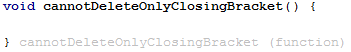
\includegraphics[width=0.50\textwidth]{screens/CannotDeleteConcreteSyntaxElements.png}
	\caption{Since the closing bracket is not part of the model, but the presentation, the bracket cannot be removed.}
	\label{fig:CannotDeleteConcreteSyntaxElements}
\end{figure}
Removing arbitrary pieces of "text" from the model is not possible. For example the closing bracket of an if statement can not be removed in isolation. The reason for this is that it is not part of the model contents (AST), but only of the presentation (concrete syntax).

\begin{figure}[H]
	\centering
	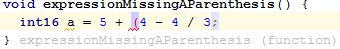
\includegraphics[width=0.5\textwidth]{screens/UnmatchedParenthesis.png}
	\caption{An unmatched parenthesis element enables more text-like editing. Inserting a closing parenthesis restructures the AST.}
	\label{fig:UnmatchedParenthesis}
\end{figure}

Designing language and editors in MPS can enable a text-like editing experience. For example,
 it is possible to design elements such as an "Unmatched Parenthesis" into your language which are not intended for the final model, but serve as an aid to enable a text-like editing experience.
 Figure~\ref{fig:UnmatchedParenthesis} shows an example of such scenario.


\subsubsection{Referencing missing items: support referencing items that have not been defined}
TODO

\subsubsection{Structure agnostic copy-paste: copy-paste works across syntax boundaries}
MPS allows selecting, copying, and pasting nodes across any language boundaries, however selection of nodes must follow the tree structure. For example, it is possible to copy 5 full statements from a selection. It is also possible to copy a node which contains a component (component language) containing a state machine (statemachine language) containing c code (c language) in action implementations. However, it is not possible to start selection halfway a node and end it halfway another one.

It is also possible to copy parts of a text-like language into a text editor. The textual content will be in the text document, but layout information and whitespace may vary.

\subsubsection{Restructuring: changing syntactic structure without typing the complete expression again.}
The example in Figure~\ref{fig:UnmatchedParenthesis} shows a model with an "Unmatched Parenthesis". Inserting a closing parenthesis will restructure the expression tree according to operator precedence rules and remove the unmatched parenthesis element.

\begin{figure}[H]
	\centering
	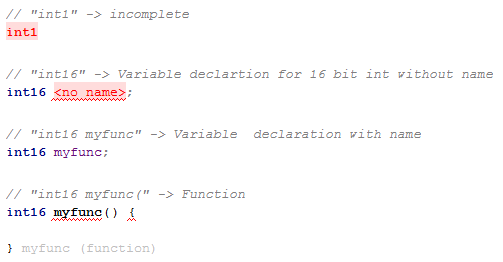
\includegraphics[width=0.5\textwidth]{screens/TypeAndRestructure.png}
	\caption{Inserting a C function in mbeddr restructures the AST as you type.}
	\label{fig:TypeAndRestructure}
\end{figure}
Figure~\ref{fig:TypeAndRestructure} shows how a C function goes through various restructurings as you type.

\subsubsection{Language demarcation: show how a combination multiple languages in one program are disambiguated}
MPS does not parse text and try to reconstruct a structure. Instead every tree node creation binds a type to a node. In case of ambiguity the user can choose which type to create. For this reason, no disambiguation is needed for the type of a node and no special demarcation markers are needed.

Similarly, reference disambiguation is ensured by default since every node has a unique ID. Although the presentation of the reference can show a human readable name/identifier, the reference refers to the node with the given ID. A side effect of this is that removing an element named "A" and creating a new element named "A" will count as a new node and existing references will be broken. If desired, these references can also be automatically be re-bound to the new node ID.

\begin{figure}[H]
	\centering
	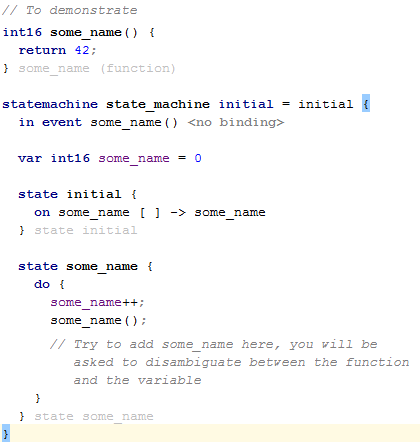
\includegraphics[width=0.5\textwidth]{screens/LanguageDemarcationAndAmbiguity.png}
	\caption{A C module, containing a state machine, containing c statements demonstrating language boundaries. The name \emph{some\_name} is heavily overloaded to demonstrate disambiguation over language boundaries.}
	\label{fig:LanguageDemarcationAndAmbiguity}
\end{figure}

Figure~\ref{fig:LanguageDemarcationAndAmbiguity} shows how various languages can be nested (c module, containing a state machine, containing c statements) and how references are resolved over these language boundaries. This example uses the same name ("some\_name") for a state, an integer, a function, and a statemachine event. But since reference insertion binds to specific ids, references over language boundaries are disambiguated by default. The screenshot does not show this, but ctrl+clicking on the references shows that all references point to the correct declaration.

\subsubsection{Delayed decisions: show when the syntactic category of an expression is determined}
At node insertion a defined concept must be inserted. However, it is possible to restructure the concepts as you type. Figure~Figure~\ref{fig:TypeAndRestructure} shows how the syntactic category changes as you type, effectively delaying the final decision and providing a text-like experience.

If a user thinks in terms of the AST instead of linear text, it is also possible to immediately insert the desired concept by using code completion or typing the alias of the desired concept. In text terms this feels similar to using a template instead of typing sequentially.

\subsubsection{End-user defined formatting: show if and how user can change the visual appearance of the program}
In MPS, end-users can be given some control over the formatting. In the visual projection, for instance,
end-users can move the nodes and the edges freely. There are some default layouts for the visual projection, but these
layouts can be changed by the end-users.

Another example of end-user defined formatting is the insertion of
empty lines in places where a statement is expected in mbeddr code. That means that the end-user can insert any number
of empty lines in the body of a function, for instance. Subsequently, the empty line can be substituted by any sub-concept of \emph{Statement}.
To achieve this behavior the \emph{Statement} concept has been declared with an editor that shows an empty line.
Moreover, the \emph{StatementList} concept contains an arbitrary number of \emph{Statement} children, and by default,
in MPS, at the press of an enter in a children collection (the statements in \emph{StatementList}), a child concept is created (\emph{Statement}).
This results in showing an empty line in the viewer because the \emph{Statement} concept is represented by an empty line.
Moreover, by default, in MPS, a concept can be substituted by any of its sub-concepts, and hence,
the \emph{Statement} concept can be replaced by any of its sub-concepts.

Thus, the amount of freedom that the end-user has in defining its own formatting
is decided, to some extent, by the language designer.

\subsubsection{Specification of default formatting: support for pretty printing}
Jetbrains MPS has a default formatting for languages. The default formatting is simply following
the structure of the abstract syntax of the language, printing the names of the instantiated concepts and
their values, and also visually showing the parent-children relationship among concepts.
An example of an expression with a defined formatting and
a default formatting is shown in Figure~\ref{fig:DefaultEditor}.

\begin{figure}[H]
	\centering
	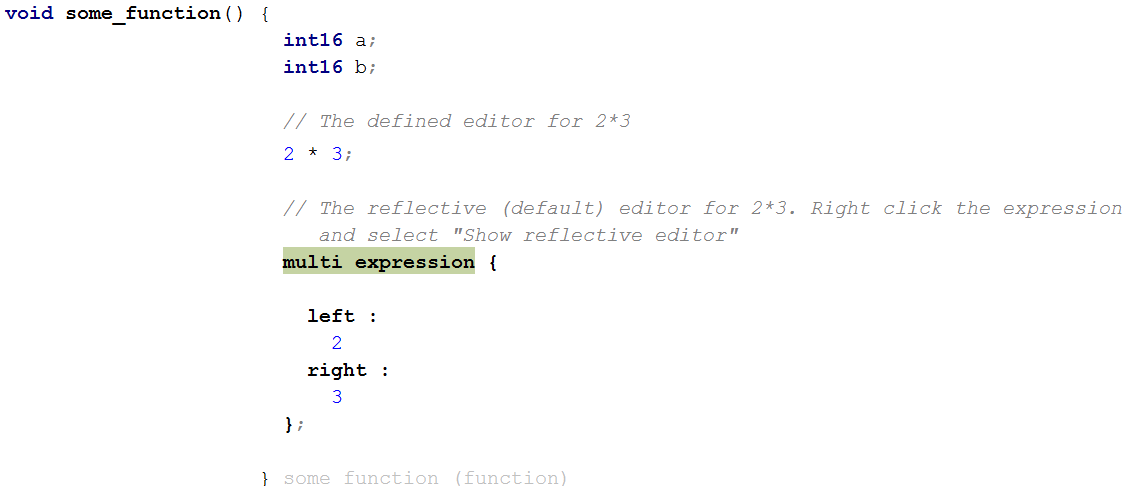
\includegraphics[width=0.50\textwidth]{screens/DefaultEditor.png}
	\caption{Defined and default formatting for a binary expression}
	\label{fig:DefaultEditor}
\end{figure}

A multitude of projections (formatting) can be defined for a given language and its concepts.
A projection is defined in an editor component, where editor cells specify the location and other attributes
of the concepts in the viewer. For instance, the editor component of the binary expression
says that the left expression (with conditional parentheses around it) is followed by a constant (the
symbol for the expression) and the right expression (again, with a conditional parentheses around it).

\begin{figure}[H]
	\centering
	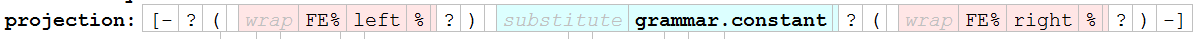
\includegraphics[width=0.50\textwidth]{screens/EditorMultiExpression.png}
	\caption{Defined editor for binary expression}
	\label{fig:DefaultEditor}
\end{figure}

Switching among projections does not modify the model itself, but only the representation of the model
on the screen.

\subsubsection{Formatting preservation: how is formatting preserved when the code is automatically restructured}
An example of a common refactoring is the introduction of a local variable in C functions \cite{voelter2014generic}.
The refactoring is triggered by selecting an expression in the body of a function, and pressing \emph{CTRL-Alt-V}.
As a result of this action, a window is prompted where the user introduces the name of the variable.
The refactoring extracts the expression, places it in a
local variable declaration and replaces all its occurrences in the body of the function with a reference to the variable.
The process can be seen in Figure~\ref{fig:IntroLocalVar}.

\begin{figure}[H]
	\centering
	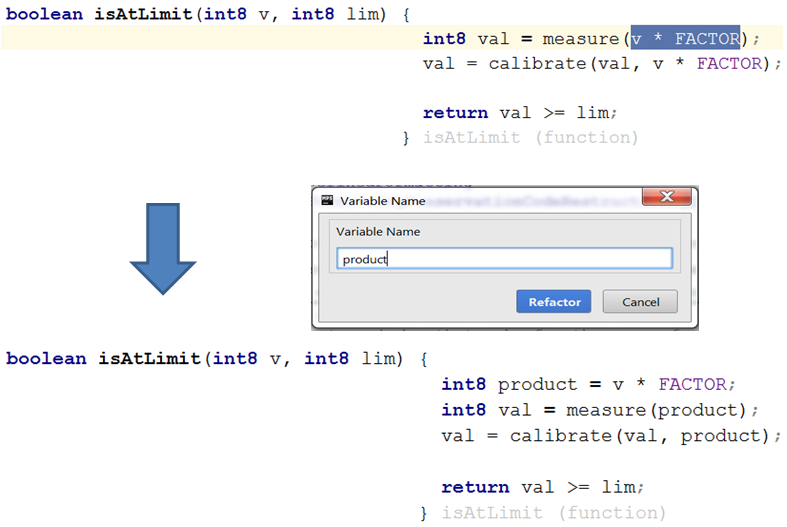
\includegraphics[width=0.50\textwidth]{screens/IntroLocalVar.png}
	\caption{Refactoring for introduction of a local variable}
	\label{fig:IntroLocalVar}
\end{figure}

The refactoring for introducing a local variable is applicable to expression concepts that have a statement as an
ancestor (see Figure~\ref{fig:RefactoringImpl}). The body of the refactoring is straightforward:
a new local variable declaration is introduced before the statement where the expression was selected and all
the occurrences of the expression are looked up and replaced. Changing an expression with a variable declaration
does not change the formatting because the change implies replacing a node in the tree with another, and the editor
component will render the new node at the specific cell, without affecting other cells. The most intrusive operation is the
introduction of the new local variable declaration in the existing statements, but this is the purpose of the
refactoring itself.

\begin{figure}[H]
	\centering
	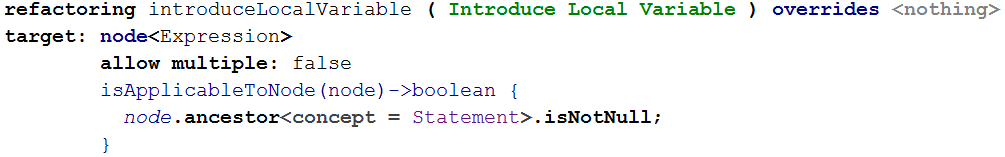
\includegraphics[width=0.50\textwidth]{screens/RefactoringImpl.png}
	\caption{Implementation header of refactoring for introduction of a local variable}
	\label{fig:RefactoringImpl}
\end{figure}

Other types of code restructuring are migration scripts in mbeddr. The situation is similar to the refactorings, the
formatting of the existing code being unchanged (unless the migration itself changes the formatting).
\subsection{Variants}

\subsection{Usability}

\subsection{Impact}

\subsection{Composability}

\subsection{Limitations}

\subsection{Uses and examples}

\subsection{Effort (best-effort)}

\subsection{Other comments}

\subsection{Artifact}

%%%%%%%%%%%%%%%%%%%%%%%%%%%%%%%%%%%%%%%%%%%%%%%%%%%%%%%%%%%%%%%%%%%%%%%%%%%%%%%
%
% Conclusions
%
%%%%%%%%%%%%%%%%%%%%%%%%%%%%%%%%%%%%%%%%%%%%%%%%%%%%%%%%%%%%%%%%%%%%%%%%%%%%%%%

\section{Conclusions}

The JetBrains MetaProgramming System has significantly evolved during the years. Nowadays it is a powerful and flexible tool that can be used to address most of the Language Engineering challenges that have been brought forward in the LWC 2016.

\textbf{Notation}
\textbf{Evolution and Reuse}
\textbf{Editing}

\section{Acknowledgements}
Our thanks go out to Markus V\"olter and Kolja Dummann from the mbeddr team for providing us with good examples from the mbeddr project. Without these, it would have taken us a lot more work to find nice examples in mbeddr or to construct such examples ourselves.

Moreover, we would like to thank Markus V\"olter for reviewing the paper and providing us with many helpful hints on how to improve it.

Finally, we would like to thank Remi Bosman from Sioux Embedded Systems for his contribution to the initial design proposal of this solution.

%% We are using the command `bibtex' from within the directory `build', thus we need
%% to go back from this directory and look for the bibliography file.
\bibliographystyle{abbrvnat}
\bibliography{../LWC2016}

\end{document}
